\chapter{Deauthentication Attack and WPA2 Handshake Capture}

This chapter outlines the practical execution of the deauthentication attack with the aim of capturing the WPA2 handshake. This method is commonly used in wireless network penetration testing to demonstrate how WPA2 can be compromised, especially when weak passwords are used.

\section{Introduction to the Deauthentication Attack}
The deauthentication attack targets connected wireless clients by sending deauthentication frames that force them to disconnect from their access point (AP). As soon as the client tries to reconnect, the WPA2 handshake is transmitted, and if captured, it can be used to attempt password recovery through brute-force or dictionary attacks.

This attack exploits the fact that deauthentication frames are not authenticated, meaning they can be easily spoofed by any device within range, making it possible for an attacker to force clients to disconnect from the network. This triggers the WPA2 handshake process, which can then be captured for further analysis.

\subsection{Tools and Software Utilized}
This section provides an overview of the tools and software employed during the practical execution of the deauthentication attack and WPA2 handshake capture. Each tool played a critical role in various stages of the attack, from configuring the network interface to analyzing the captured handshake.

\subsubsection{Airmon-ng}
Part of the `aircrack-ng` suite, `airmon-ng` is a tool used to enable and manage monitor mode on wireless network interfaces. In this experiment, it was employed to switch the wireless adapter into monitor mode, allowing it to capture all wireless traffic within range. Additionally, it was used to terminate interfering processes to ensure a smooth operation during packet capture.

\subsubsection{Airodump-ng}
`Airodump-ng` is another utility within the `aircrack-ng` suite, designed for packet capture and real-time analysis of wireless traffic. It was instrumental in scanning for nearby networks, identifying the target access point, and capturing the WPA2 handshake during the attack.

\subsubsection{Aireplay-ng}
`Aireplay-ng` is a packet injection tool used to perform various wireless network attacks, including deauthentication attacks. In this experiment, it was utilized to send deauthentication frames to force connected clients to disconnect from the target access point, thereby triggering the WPA2 handshake.

\subsubsection{Aircrack-ng}
The `aircrack-ng` tool is the centerpiece of the suite, specializing in wireless network password cracking. In this scenario, it was used to execute the dictionary attack on the captured WPA2 handshake. By iterating through the entries in the `rockyou.txt` wordlist, `aircrack-ng` successfully recovered the network password.

\subsubsection{Wireshark}
Wireshark is a versatile network protocol analyzer used for inspecting captured network traffic in detail. After capturing the WPA2 handshake, Wireshark was employed to verify the integrity of the handshake and confirm that all necessary packets were captured correctly.

\subsubsection{RockYou Dictionary}
The `rockyou.txt` dictionary is a widely known wordlist containing millions of commonly used passwords. It served as the dictionary for the password-cracking phase, highlighting the risks associated with weak and commonly used passwords.

Each of these tools contributed to the successful execution of the attack, from capturing wireless traffic to analyzing and recovering the network password. Their combined functionality underscores the importance of understanding and mitigating these vulnerabilities in wireless network security.


\section{Objective and Methodology for Capturing the WPA2 Handshake}
The primary goal of this section is to capture the WPA2 handshake between a client and the AP using the deauthentication attack. The following steps outline the process and the commands used for execution:

\begin{enumerate}
    \item \textbf{Switching the Network Interface to Monitor Mode:} The first step in preparing for the deauthentication attack is to enable monitor mode on the wireless adapter, which allows the interface to capture all wireless traffic within range. As illustrated in Figure \ref{fig:wlanmon}, I began by checking the current state of the wireless interface using the command \textit{iwconfig}. To ensure that no processes would interfere with the monitor mode, I terminated any conflicting processes using the command \textit{sudo airmon-ng check kill}. Finally, I switched the wireless card into monitor mode with the command \textit{sudo airmon-ng start wlan0}, which reconfigures the adapter from managed to monitor mode, enabling it to capture all nearby wireless packets.

    \begin{figure}[h!]
        \centering
        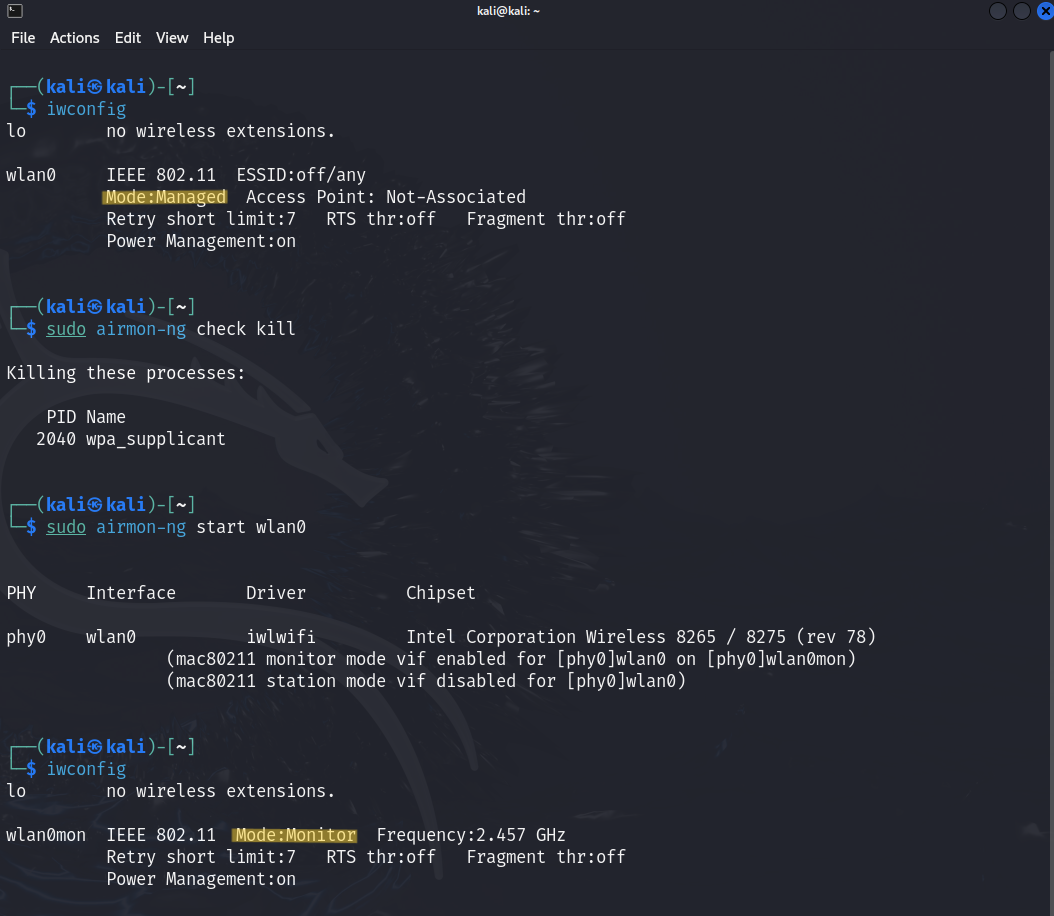
\includegraphics[width=0.8\linewidth]{images/wlanmon.png}
        \caption{Monitor mode enabled on the wireless card.}
        \label{fig:wlanmon}
    \end{figure}

    \item \textbf{Scanning for Nearby Networks:} Once the network interface was in monitor mode, the next step was to scan for nearby wireless networks. This was accomplished using the command \textit{sudo airodump-ng wlan0mon}.

    As shown in Figure \ref{fig:networklist}, this command provides a list of all available access points, displaying details such as the BSSID (MAC address), channel, encryption type, and the number of connected clients. From this list, I was able to identify the target network, along with its corresponding BSSID and channel.

    \begin{figure}[h!]
        \centering
        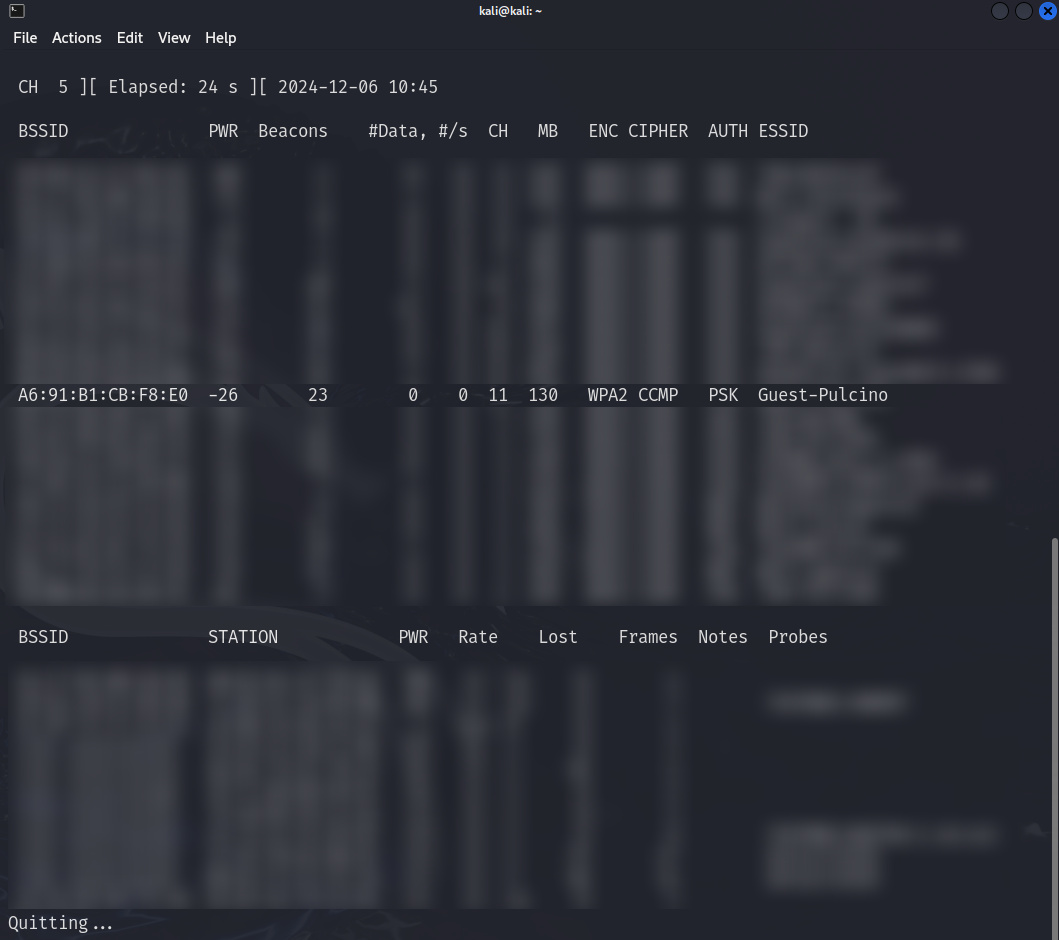
\includegraphics[width=0.8\linewidth]{images/networklist.png}
        \caption{List of nearby networks and stations.}
        \label{fig:networklist}
    \end{figure}

    At this stage, I had successfully identified the BSSID and channel of my target network.

    \item \textbf{Identifying the Target Network:} After identifying the target network, the next step was to focus the attack on the specific channel used by the target access point. To filter the results and capture only the traffic from the target network, I used the following command: \textit{"sudo airodump-ng --bssid A6:91:B1:CB:F8:E0 -c 11 -w wificapture wlan0"}. In this command, the \textit{-w wificapture} flag specifies the filename where the captured handshake will be saved, and the \textit{-c 11} flag ensures that only traffic on channel 11, where the target AP operates, is captured. The results are displayed in Figure \ref{fig:handshakelistening}.

    \begin{figure}[h!]
        \centering
        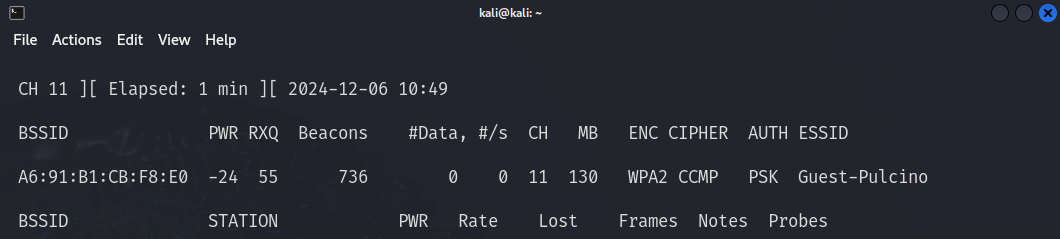
\includegraphics[width=0.8\linewidth]{images/handshakelistening.png}
        \caption{Listening for the handshake on the target network.}
        \label{fig:handshakelistening}
    \end{figure}

    \item \textbf{Sending Deauthentication Frames:} With the target network identified and the capture in progress, the next step was to send deauthentication frames to disconnect any connected clients from the access point. As shown in Figure \ref{fig:deauth}, this was achieved using the following command: \textit{"sudo aireplay-ng --deauth 0 -a A6:91:B1:CB:F8:E7 wlan0mon"}. The \textit{--deauth 0} flag indicates that deauthentication packets will be sent indefinitely (until manually stopped). These frames force the connected devices to disconnect and attempt to reconnect, which triggers the WPA2 handshake.

    \begin{figure}[h!]
        \centering
        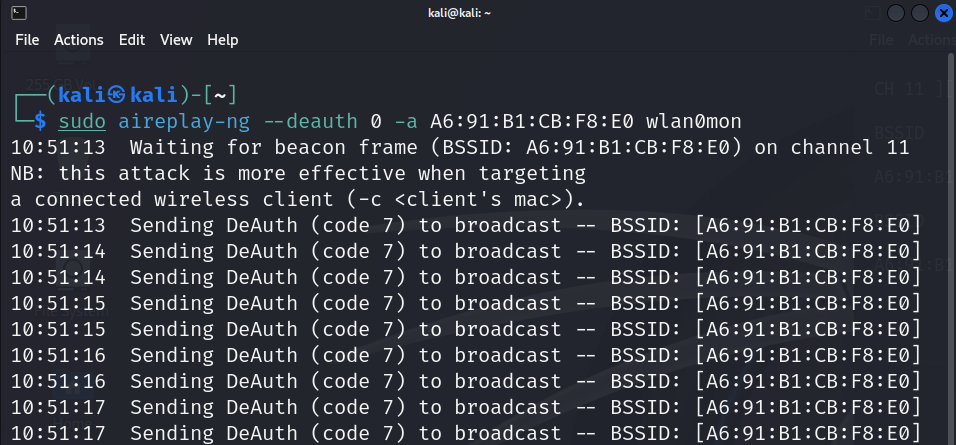
\includegraphics[width=0.8\linewidth]{images/dauth.png}
        \caption{Deauthentication packets being sent.}
        \label{fig:deauth}
    \end{figure}

    \item \textbf{Capturing the WPA2 Handshake:} When a client attempts to reconnect to the access point, the WPA2 handshake is triggered and captured by the \textit{airodump-ng} tool. This handshake is crucial for subsequent analysis. Once the handshake capture is complete, the tool provides confirmation in the form of output, as shown in Figure \ref{fig:handshakecaputred}.

    \begin{figure}[h!]
        \centering
        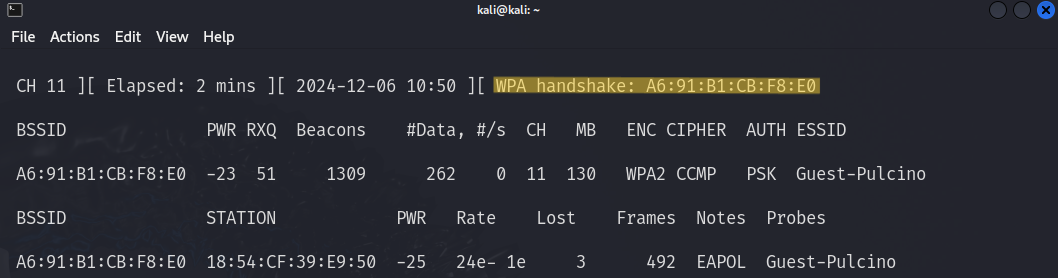
\includegraphics[width=0.8\linewidth]{images/handshakecaptured.png}
        \caption{WPA2 handshake successfully captured.}
        \label{fig:handshakecaputred}
    \end{figure}
    
    The captured handshake is then saved to the specified file, ready for further analysis or potential use in an attack.

    \item \textbf{Analyzing the Handshake:} The captured handshake was analyzed using \texttt{Wireshark} to verify its completeness and to understand the cryptographic exchanges between the client and the AP. As outlined in the theoretical section, the WPA2 handshake consists of four messages that establish the Pairwise Transient Key (PTK) and the Group Temporal Key (GTK), ensuring secure communication between the two parties.

\begin{enumerate}
    \item \textbf{Message 1:} The AP sends a random nonce (\texttt{ANONCE}) to the client. This nonce, shown in Figure \ref{fig:msg1}, is crucial for the client to derive the PTK using the pre-shared key (PSK) and other parameters.
    \begin{figure}[h!]
        \centering
        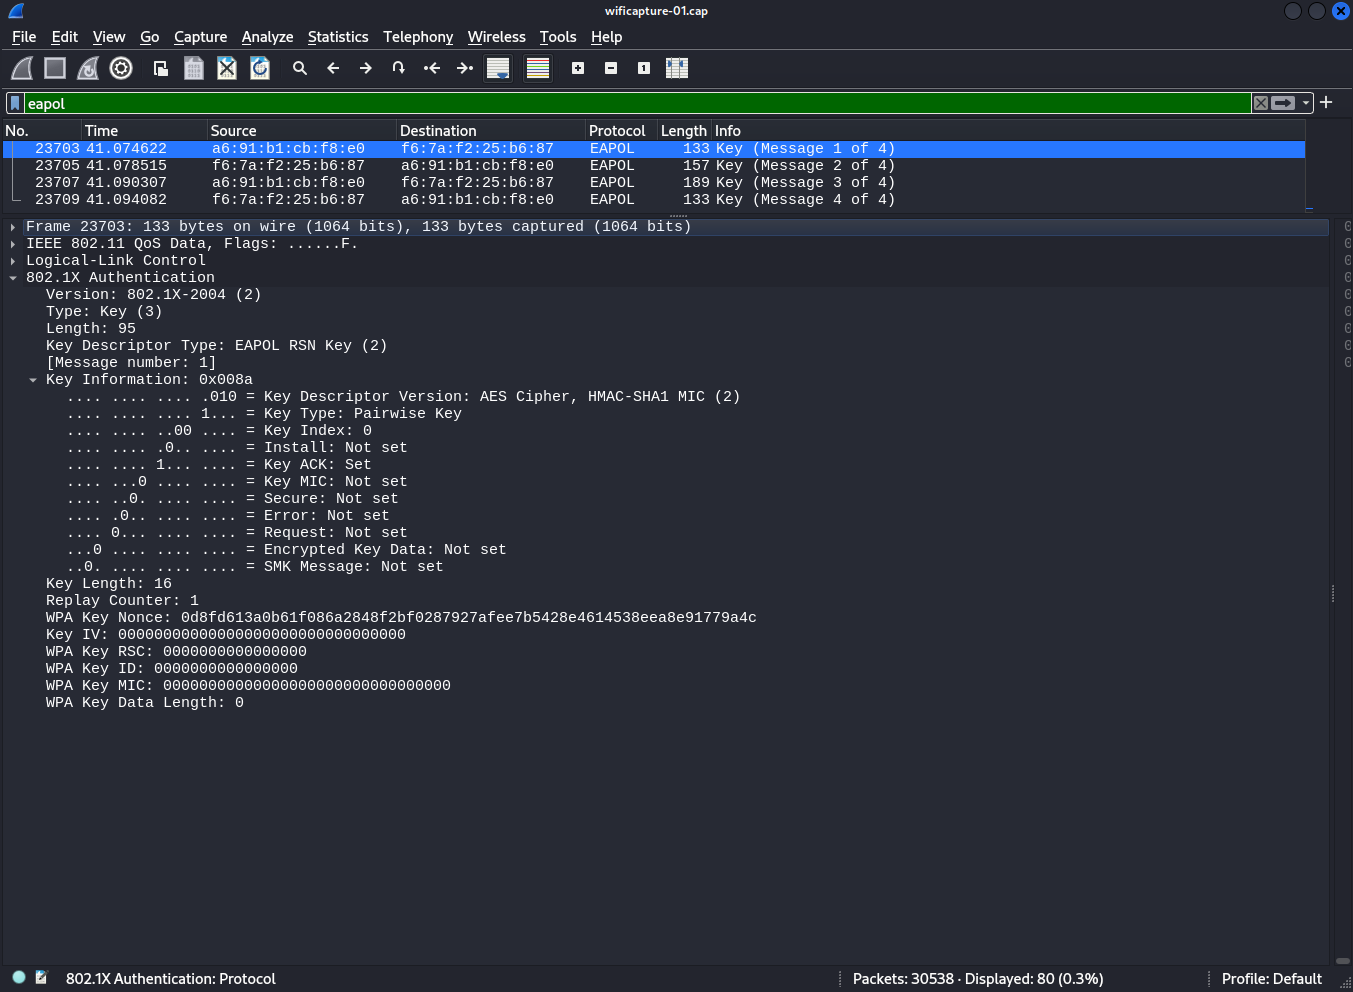
\includegraphics[width=0.8\linewidth]{images/msg1.png}
        \caption{Message 1: AP sending ANONCE to the client.}
        \label{fig:msg1}
    \end{figure}

    \item \textbf{Message 2:} The client responds with its own nonce (\texttt{SNONCE}) and a Message Integrity Code (MIC) to ensure the integrity of the exchange. As depicted in Figure \ref{fig:msg2}, this step confirms the client’s identity and provides the AP with the data needed to compute the PTK.
    \begin{figure}[h!]
        \centering
        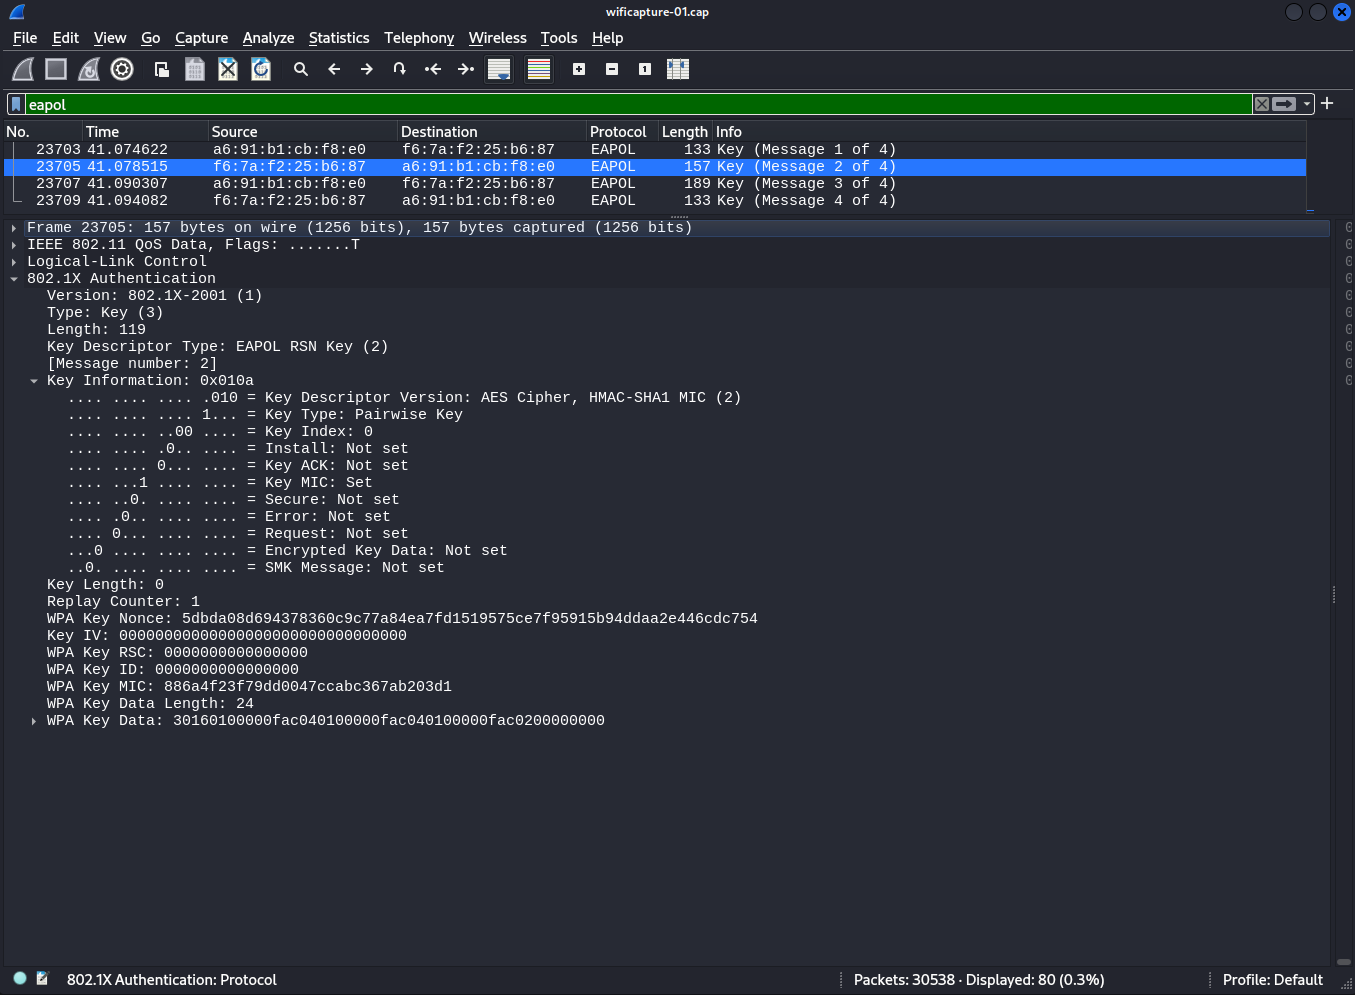
\includegraphics[width=0.8\linewidth]{images/msg2.png}
        \caption{Message 2: Client sending SNONCE and MIC to the AP.}
        \label{fig:msg2}
    \end{figure}

    \item \textbf{Message 3:} The AP transmits the Group Temporal Key (GTK) to the client, ensuring that all clients on the network can securely communicate in multicast and broadcast traffic. This can be seen in Figure \ref{fig:msg3}.
    \begin{figure}[h!]
        \centering
        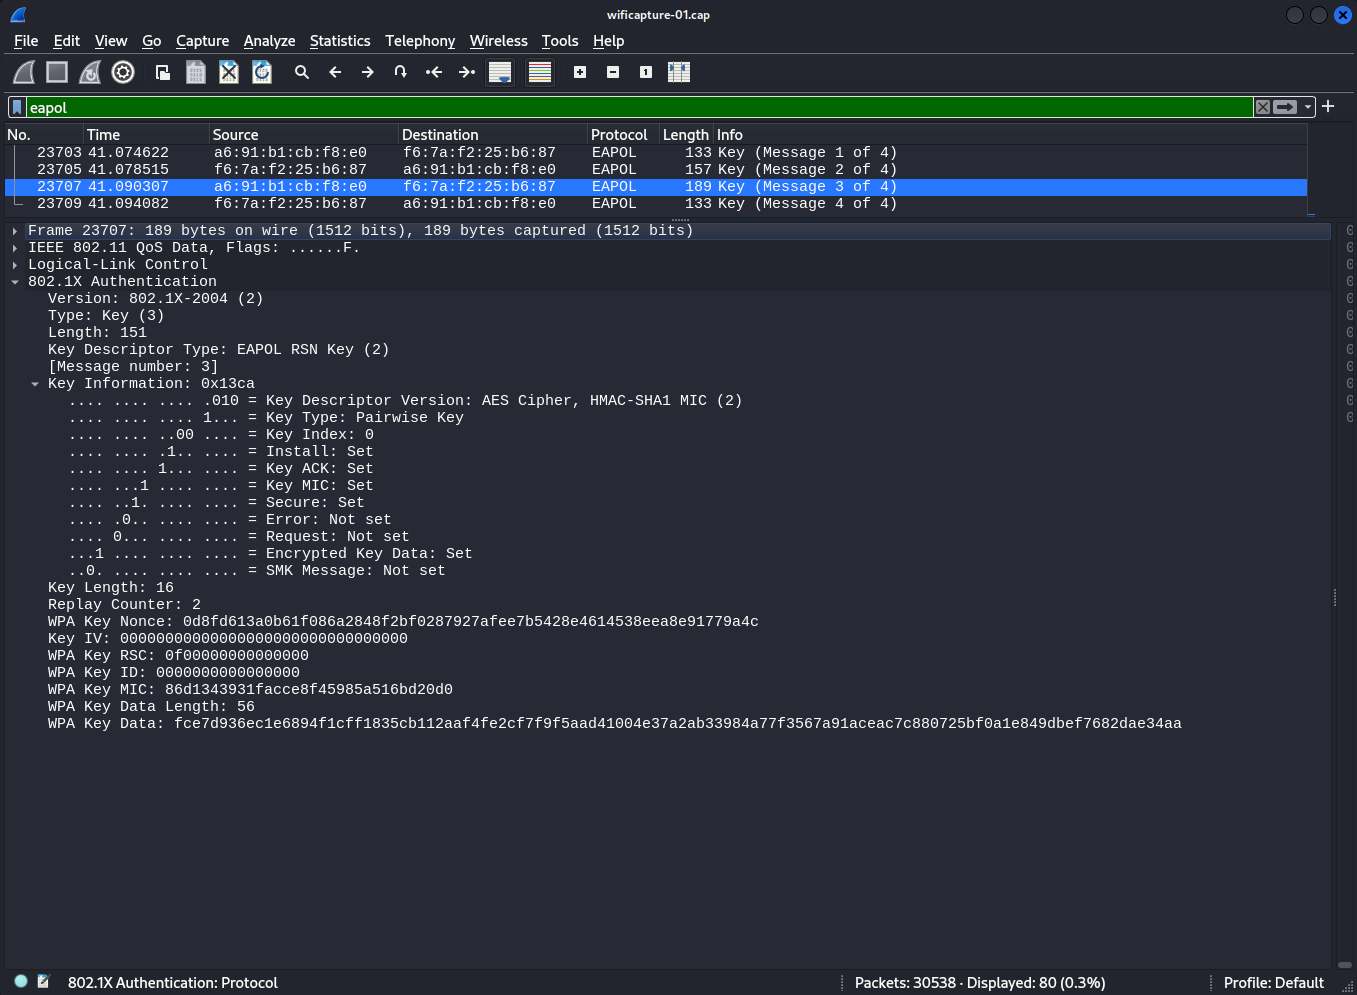
\includegraphics[width=0.8\linewidth]{images/msg3.png}
        \caption{Message 3: AP sending GTK to the client.}
        \label{fig:msg3}
    \end{figure}

    \item \textbf{Message 4:} The client sends a final acknowledgment to the AP, confirming the installation of the PTK and GTK. This step, illustrated in Figure \ref{fig:msg4}, completes the handshake process, establishing a secure communication channel.
    \begin{figure}[h!]
        \centering
        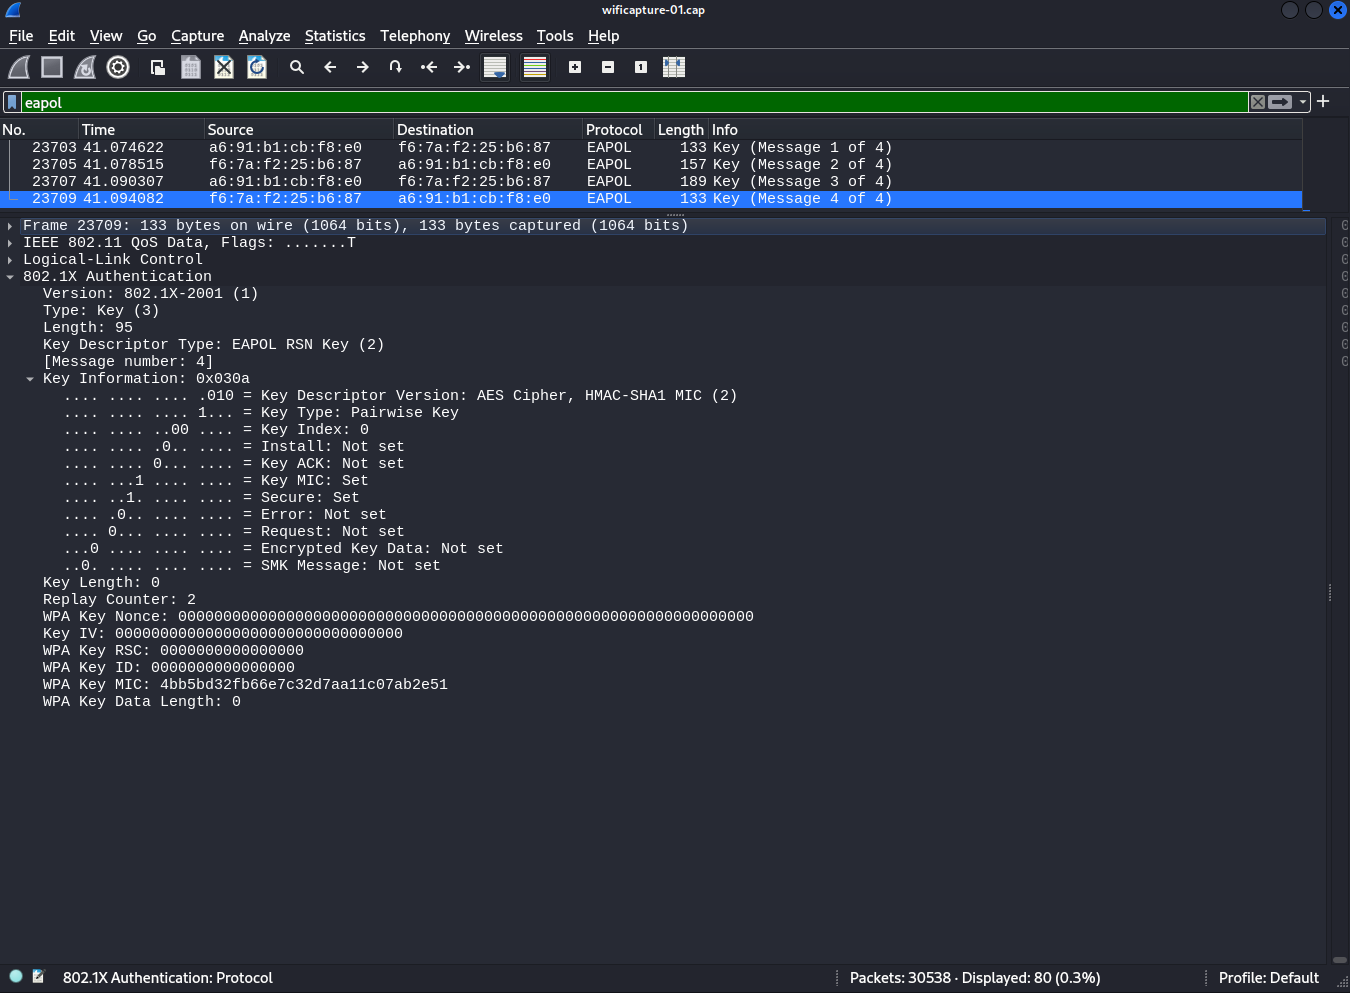
\includegraphics[width=0.8\linewidth]{images/msg4.png}
        \caption{Message 4: Client confirming the handshake completion.}
        \label{fig:msg4}
    \end{figure}
\end{enumerate}

By examining these messages in \texttt{Wireshark}, it was possible to confirm the integrity of the handshake. Each message plays a distinct role in ensuring a secure and authenticated connection, as described in the theoretical overview of the WPA2 Four-Way Handshake. The detailed inspection of the captured packets reinforced the understanding of the cryptographic mechanisms at play, providing valuable insights into the vulnerabilities associated with weak pre-shared keys.


    \item \textbf{Performing a Dictionary Attack:} Once the handshake was successfully captured, I proceeded with the dictionary attack to attempt to recover the password. Here’s the series of steps I followed:

    \begin{enumerate}
        \item \textbf{Extracting the RockYou Dictionary:} The first step was to extract the \texttt{rockyou.txt} dictionary file from its compressed archive. This was done using the command \textit{gunzip /usr/share/wordlists/rockyou.txt.gz}
        This command unzipped the compressed file, making the dictionary ready for use.

        \item \textbf{Initiating the Dictionary Attack:} With the handshake file and the dictionary prepared, I used the \texttt{aircrack-ng} tool to perform the attack. The command used was \textit{aircrack-ng wificapture.cap -w /usr/share/wordlists/rockyou.txt}
        
        Where:
        \begin{itemize}
            \item \texttt{-w}: Specifies the path to the wordlist (\texttt{rockyou.txt} in this case).
            \item \texttt{wificapture.cap}: The file containing the captured handshake.
        \end{itemize}

        \begin{figure}[h!]
            \centering
            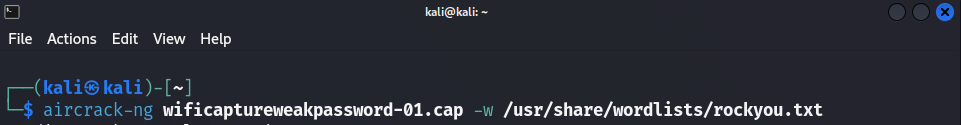
\includegraphics[width=0.8\linewidth]{images/rockyoucommand.png}
            \caption{Dictionary brute-force attack in progress.}
            \label{fig:rockyoucommand}
        \end{figure}

        \item \textbf{Waiting for the Process to Complete:} The \texttt{aircrack-ng} tool iteratively tested each password in the dictionary against the handshake data. Since the target network password was deliberately set to a simple passphrase for demonstration purposes, the tool successfully identified the password in a short amount of time. The output from \texttt{aircrack-ng} confirmed the recovered password, as shown in Figure \ref{fig:passwordfound}.

        \begin{figure}[h!]
            \centering
            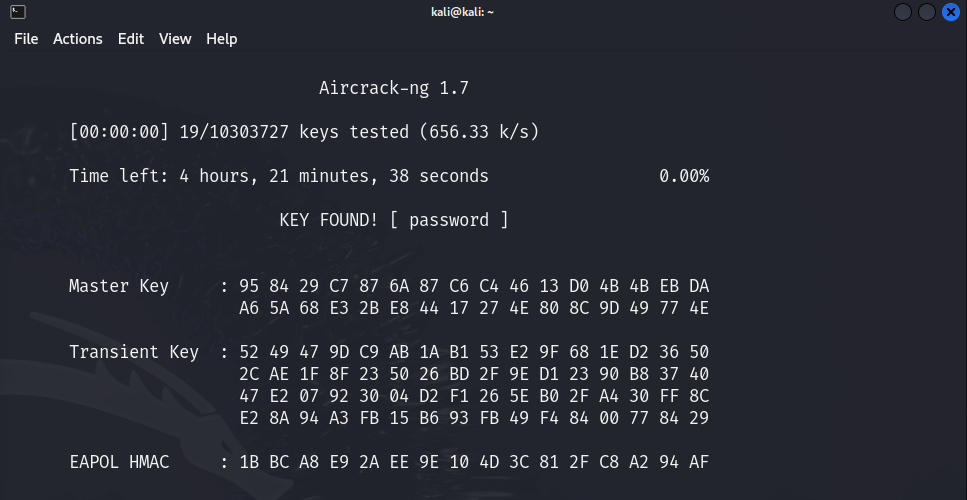
\includegraphics[width=0.8\linewidth]{images/passwordfound.png}
            \caption{Password successfully recovered using the dictionary attack.}
            \label{fig:passwordfound}
        \end{figure}
    \end{enumerate}
    
    This demonstration highlights the effectiveness of dictionary attacks against weak passwords and underscores the importance of using strong, unique passphrases to secure WPA2 networks.
    
\end{enumerate}


\section{Results and Analysis}
The deauthentication attack proved to be highly effective in demonstrating the vulnerabilities of WPA2 networks when weak passwords are employed. By sending deauthentication frames, the target client was successfully disconnected from the network. This action forced the client to attempt reconnection, triggering the WPA2 handshake. Using the `airodump-ng` tool, the handshake was captured with ease, confirming the effectiveness of this method in acquiring essential data for further analysis.

The next phase involved performing a dictionary attack on the captured handshake using `aircrack-ng`. The process relied on the `rockyou.txt` wordlist, a widely used dictionary for such purposes. Within a short period, the tool successfully recovered the network password. This success was largely due to the deliberately chosen weak password used in the demonstration, highlighting how easily poorly selected credentials can be compromised.

Overall, the experiment revealed that WPA2 networks with weak passwords are highly susceptible to such attacks. It underscores the importance of strong security measures to protect wireless communications from unauthorized access.

\section{Conclusion}
This study highlights the inherent vulnerabilities in WPA2 networks when secured with weak or easily guessable passwords. The deauthentication attack exploited the unauthenticated nature of deauthentication frames to disconnect a client, capturing the WPA2 handshake during its reconnection attempt. The subsequent dictionary attack demonstrated how attackers can leverage captured handshakes to recover passwords when weak credentials are used.

The results emphasize the necessity of adopting robust security practices, such as choosing strong, complex, and unique passwords to secure wireless networks. Additionally, the implementation of advanced security protocols like WPA3, which mitigates many of the weaknesses inherent in WPA2, is vital to ensuring the resilience of modern networks.

Through this practical demonstration, the chapter sheds light on the potential risks faced by wireless networks and the critical need for both users and administrators to prioritize security. A proactive approach to network configuration and encryption standards can significantly reduce the likelihood of such attacks succeeding.

